% This file was created with tikzplotlib v0.10.1.
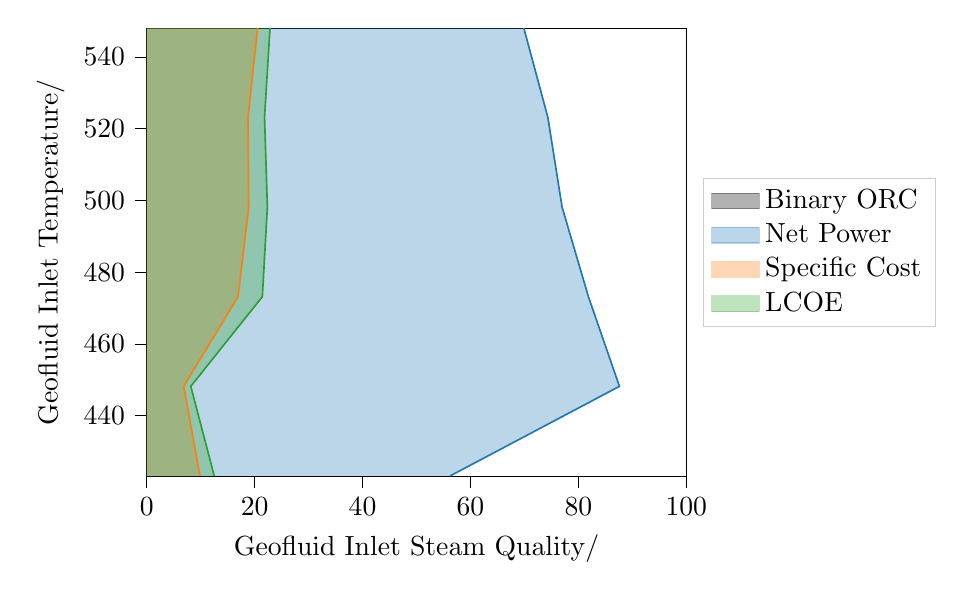
\begin{tikzpicture}

\definecolor{darkgray176}{RGB}{176,176,176}
\definecolor{darkorange25512714}{RGB}{255,127,14}
\definecolor{forestgreen4416044}{RGB}{44,160,44}
\definecolor{lightgray204}{RGB}{204,204,204}
\definecolor{steelblue31119180}{RGB}{31,119,180}

\begin{axis}[
legend cell align={left},
legend style={
  fill opacity=0.8,
  draw opacity=1,
  text opacity=1,
  at={(1.03,0.5)},
  anchor=west,
  draw=lightgray204
},
tick align=outside,
tick pos=left,
x grid style={darkgray176},
xlabel={Geofluid Inlet Steam Quality/\unit{\percent}},
xmin=0, xmax=100,
xtick style={color=black},
y grid style={darkgray176},
ylabel={Geofluid Inlet Temperature/\unit{\K}},
ymin=423, ymax=548,
ytick style={color=black}
]
\path [draw=black, fill=black, opacity=0.3]
(axis cs:0,551)
--(axis cs:0,550)
--(axis cs:100,550)
--(axis cs:100,551)
--(axis cs:100,551)
--(axis cs:0,551)
--cycle;
\addlegendimage{area legend, draw=black, fill=black, opacity=0.3}
\addlegendentry{Binary ORC}

\path [fill=steelblue31119180, fill opacity=0.3]
(axis cs:0,548.15)
--(axis cs:69.8700824552182,548.15)
--(axis cs:74.3434951467281,523.15)
--(axis cs:76.9746128225481,498.15)
--(axis cs:81.858282772291,473.15)
--(axis cs:87.6035000467469,448.15)
--(axis cs:56.2118978404422,423.15)
--(axis cs:0,423.15)
--(axis cs:0,423.15)
--(axis cs:0,448.15)
--(axis cs:0,473.15)
--(axis cs:0,498.15)
--(axis cs:0,523.15)
--(axis cs:0,548.15)
--cycle;

\path [fill=darkorange25512714, fill opacity=0.3]
(axis cs:0,548.15)
--(axis cs:20.5762377366254,548.15)
--(axis cs:18.7802120957028,523.15)
--(axis cs:18.9135989940054,498.15)
--(axis cs:16.9385562572759,473.15)
--(axis cs:6.87075617227907,448.15)
--(axis cs:9.88045623429895,423.15)
--(axis cs:0,423.15)
--(axis cs:0,423.15)
--(axis cs:0,448.15)
--(axis cs:0,473.15)
--(axis cs:0,498.15)
--(axis cs:0,523.15)
--(axis cs:0,548.15)
--cycle;

\path [fill=forestgreen4416044, fill opacity=0.3]
(axis cs:0,548.15)
--(axis cs:22.8608023758107,548.15)
--(axis cs:21.846254027533,523.15)
--(axis cs:22.3651676590047,498.15)
--(axis cs:21.4380729926894,473.15)
--(axis cs:8.17474478116097,448.15)
--(axis cs:12.5271176272021,423.15)
--(axis cs:0,423.15)
--(axis cs:0,423.15)
--(axis cs:0,448.15)
--(axis cs:0,473.15)
--(axis cs:0,498.15)
--(axis cs:0,523.15)
--(axis cs:0,548.15)
--cycle;

\addlegendimage{area legend, draw=steelblue31119180, fill=steelblue31119180, opacity=0.3}
\addplot [semithick, steelblue31119180, forget plot]
table {%
69.8700824552182 548.15
74.3434951467281 523.15
76.9746128225481 498.15
81.858282772291 473.15
87.6035000467469 448.15
56.2118978404422 423.15
};
\addlegendentry{Net Power}
\addlegendimage{area legend, draw=darkorange25512714, fill=darkorange25512714, opacity=0.3}
\addplot [semithick, darkorange25512714, forget plot]
table {%
20.5762377366254 548.15
18.7802120957028 523.15
18.9135989940054 498.15
16.9385562572759 473.15
6.87075617227907 448.15
9.88045623429895 423.15
};
\addlegendentry{Specific Cost}
\addlegendimage{area legend, draw=forestgreen4416044, fill=forestgreen4416044, opacity=0.3}
\addplot [semithick, forestgreen4416044, forget plot]
table {%
22.8608023758107 548.15
21.846254027533 523.15
22.3651676590047 498.15
21.4380729926894 473.15
8.17474478116097 448.15
12.5271176272021 423.15
};
\addlegendentry{LCOE}
\end{axis}

\end{tikzpicture}
